\documentclass[12pt]{beamer}
\usepackage[czech]{babel}
\usepackage[longend, ruled]{algorithm2e}
\usepackage{graphicx}
\usepackage{grffile}

\usetheme{Madrid}


\title[Řadící algoritmy] %optional
{Řadicí algoritmy}
\subtitle{Shell sort}
\author[Vadim] % (optional)
{\large G.~Vadim\inst{1}}

\institute[VUT FIT] % (optional)
{
  \inst{1}%
  \textsc{Vysoké učeni technické v Brně\\
  Fakulta Informačních technologií}
}

\date[ITY 2022] % (optional)
{\\\large Typografie a publikování, \today}

\begin{document}
\frame{\titlepage}

\begin{frame}
    \frametitle{Úvod \& motivace}
    \bigskip
    \hspace*{20pt}\texttt{Algoritmus řazení} je algoritmus, který řadí prvky seznamu do pořadí. Efektivní řazení je důležité pro optimalizaci účinnosti jiných algoritmů, které vyžadují, aby vstupní data byla v seřazených seznamech.
    
    %Algoritmus řazení se používá k uspořádání prvků pole/seznamu v určitém pořadí. K dokončení této operace lze použít různé třídicí algoritmy.  A můžeme použít jakýkoli algoritmus založený na požadavku.
    \begin{figure}[htb]
    \centering
    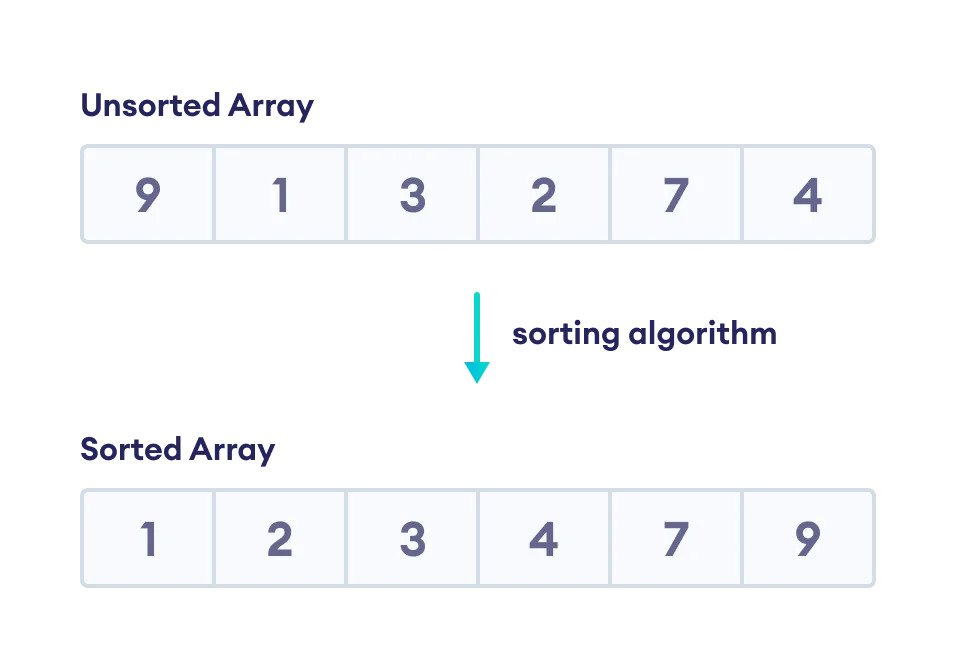
\includegraphics[scale=0.225]{unsort-sort.jpg}
    
    \end{figure}
\end{frame}

\begin{frame}
    \frametitle{Klasifikace}
    
        \fontsize{14pt}{12pt}\selectfont
        \hspace*{20pt}\texttt{Algoritmus řazení} lze klasifikovat podle:
        \bigskip
        
        \emph{
        \begin{itemize}
            \fontsize{12pt}{12pt}\selectfont
            \setlength{\itemindent}{2em}
            \item Výpočetní složitostí
            \item Využití paměti \textnormal{(a dalších počítačových zdrojů)}
            \item Rekurzivity
            \item Stability
            \item Zda je nebo není porovnávacím řazením
            \item Zda je sériový nebo paralelní
            \item Adaptability
            \item Online přístupu
        \end{itemize}
        }
    
    
    
    
\end{frame}


\begin{frame}
    \frametitle{Přehled řadicích algoritmů}
    
    \begin{columns}[T] % align columns
    \begin{column}{.48\textwidth}
        \bigskip
        \emph{
        \begin{itemize}
        \setlength{\itemindent}{3em}
            \item Bubble sort
            \item Selection sort
            \item Insertion sort
            \item Merge sort
            \item \alert<2>{Shell sort}
            \item Quicksort
            \item Counting sort
            \item Radix sort
            \item Bucket sort
            \item Heap sort
        \end{itemize}
        }
    \end{column}%
    
    \hfill%
    \begin{column}{.48\textwidth}
        
        \begin{figure}[htb]
            \centering
            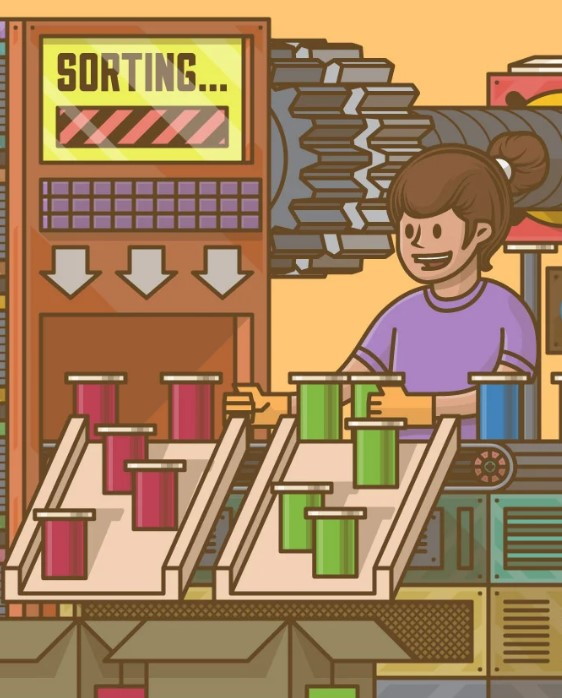
\includegraphics[scale=0.35]{sorting.jpg}
            
        \end{figure}
    \end{column}%
    
    \end{columns}
    
    
\end{frame}

\begin{frame}
    \frametitle{Shell sort}
    \fontsize{10pt}{12pt}\selectfont
    
    \hspace*{20pt}\texttt{Shell sort }je zobecněná verze algoritmu řazení vložení (\uv{insertion sort}).
    Nejprve seřadí prvky, které jsou od sebe daleko, a postupně zkracuje interval mezi prvky, které mají být seřazeny.
    
    \vspace{\baselineskip}
    \hspace*{20pt}Interval je zkrácen na základě použité sekvence. Některé z optimálních sekvencí, které lze použít v algoritmu řazení Shellu, jsou:
    \vspace{\baselineskip}
    
    \begin{itemize}
    \setlength{\itemindent}{3em}
        \item Původní Shellová sekvence: \emph{N/2, N/4, \dots, 1}
        \item Knuthový přírůstky: \emph{1, 4, 13, \dots, (3k – 1)/2}
        \item Sedgewickový přírůstky: \emph{1, 8, 23, 77, 281, 107,\dots,4j+1+3*2j+1}
        \item Hibbardový přírůstky: \emph{1, 3, 7, 15, 31, 63, 127, 255, 511\dots}
        \item Přírůstek Papernova \& Staseviche: \emph{1, 3, 5, 9, 17, 33, 65\dots}
        \item Pratt: \emph{1, 2, 3, 4, 6, 9, 8, 12, 18, 27, 16, 24, 36, 54, 81\dots}
    \end{itemize}   
\end{frame}

\begin{frame}
    \frametitle{Shell sort. Motivace}
    \hspace*{20pt}\texttt{Shell sort }se používá, když:
    \bigskip
    \fontsize{10pt}{12pt}\selectfont

    \emph{
    \begin{itemize}
        \item volání zásobníku je velká režie.
        \item rekurze překročí určitý limit.
        \item insertion sort nefunguje dobře, protože jsou blízké prvky daleko od sebe.
    \end{itemize}
    }
    \bigskip
    
    \hspace*{20pt}\texttt{Shell sort }pomáhá při zmenšování vzdálenosti mezi blízkými prvky.
    
    \hspace*{20pt}Tím se sníží počet prohození, která je třeba provést.
    
    \fontsize{12pt}{12pt}\selectfont
    \bigskip
    \begin{block}{Aplikace}
        \hspace*{20pt}\emph{Knihovna uClibc a kompresor bzip2 používají Shell sort.}
    \end{block}
    
    
\end{frame}

\begin{frame}
    \frametitle{Shell sort. První iterace}
    \fontsize{10pt}{12pt}\selectfont
    \begin{block}{Předpokládejme, že potřebujeme seřadit následující pole.}
        
        \begin{figure}[htb]
        \centering
        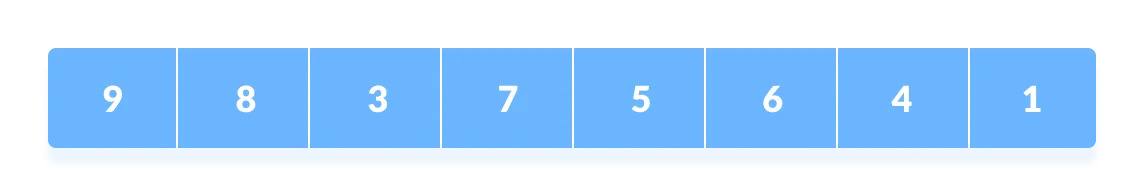
\includegraphics[scale=0.175]{1.jpg}
        
        \end{figure}
    \end{block}
    \begin{enumerate}
    %\setlength{\itemindent}{3em}
        \item Jako intervaly v našem algoritmu použijeme původní posloupnost $(N/2, N/4, ...1)$.
        
        \item Pokud je velikost pole $N = 8$, pak se v první smyčce porovnají prvky ležící v intervalu $N/2 = 4$ a prohodí se, pokud nejsou v pořadí.
        \item $0.$ prvek se porovná se $4.$ prvkem.
        \item Je-li $0.$ prvek větší než $4.$ prvek, pak se $0.$ prvek (tj. větší prvek) se uloží na $4.$ pozici a $4.$ prvek se uloží na $0.$ pozici.
    \end{enumerate}
\end{frame}


\begin{frame}
    \frametitle{Shell sort. První iterace}
    \fontsize{14pt}{12pt}\selectfont
    \centering
    \begin{block}{Interval N/2}
    Tento postup pokračuje u všech zbývajících prvků.
    \end{block}
    
    \begin{figure}[htb]
    
    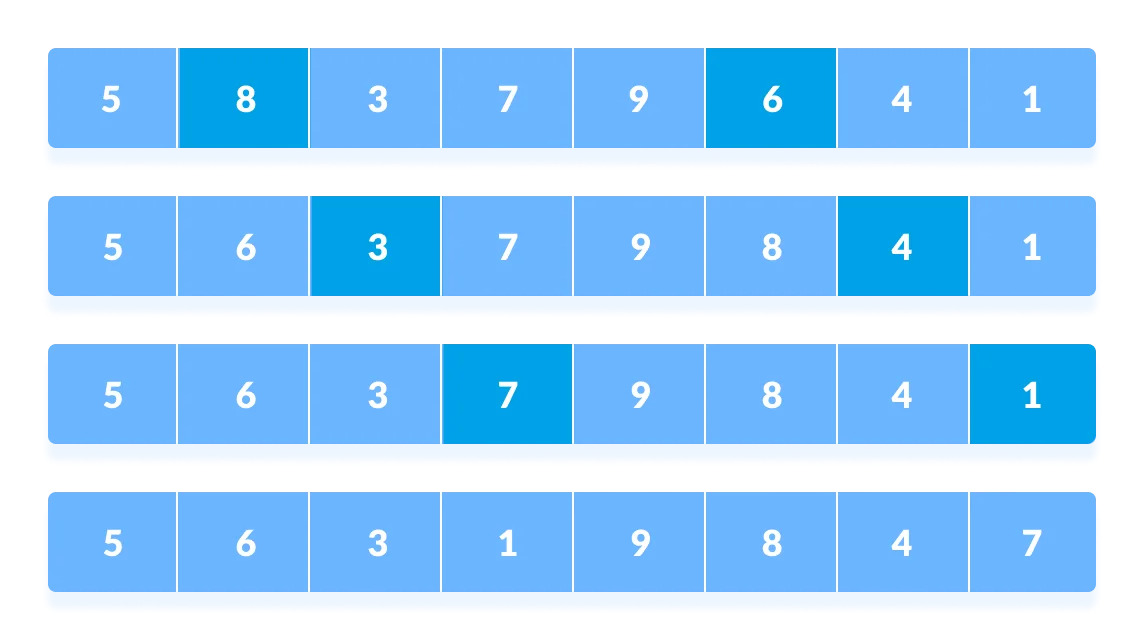
\includegraphics[scale=0.225]{2.jpg}
    
    \end{figure}
    
\end{frame}

\begin{frame}
    \frametitle{Shell sort. Druhá iterace}
    \fontsize{12pt}{12pt}\selectfont
    \begin{block}{Interval N/4}
    Ve druhé interací je vybrán interval N/4 = 8/4 = 2 a opět jsou seřazeny prvky ležící v těchto intervalech.
    \end{block}
    
    \begin{figure}[htb]
        \centering
        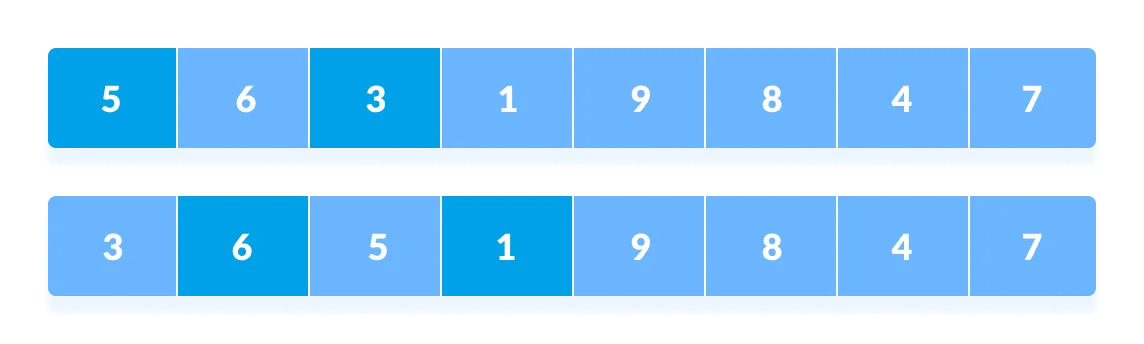
\includegraphics[scale=0.2]{3.jpg}
        
        {\Huge\dots}
        \vspace{\baselineskip}
        
        
\includegraphics[scale=0.2]{4.jpg}
    \end{figure}
    
\end{frame}

\begin{frame}
    \frametitle{Shell sort. Třetí iterace}
    \fontsize{12pt}{12pt}\selectfont
    \begin{block}{Interval N/8}
    Nakonec, když je interval N/8 = 8/8 =1, pak jsou seřazeny prvky pole ležící v intervalu 1. Pole je nyní kompletně seřazené.
    \end{block}
    
    \begin{figure}[htb]
        \centering
        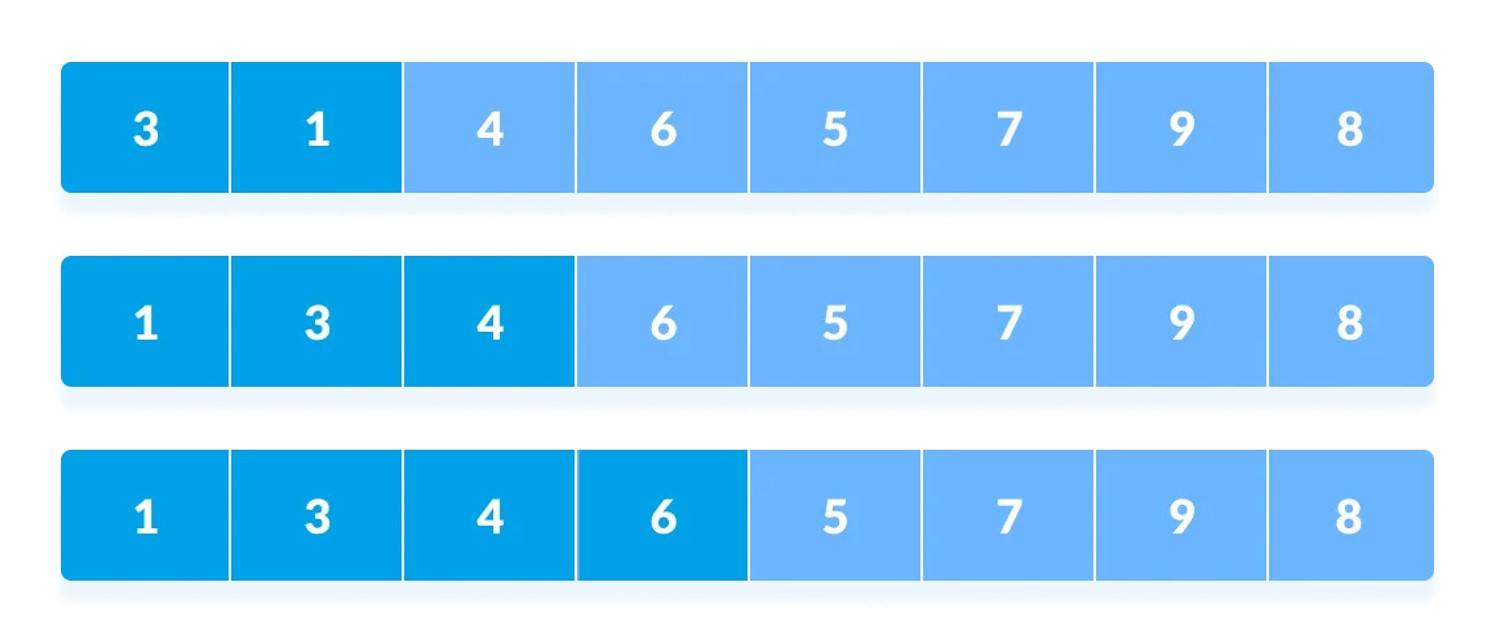
\includegraphics[scale=0.2]{5.jpg}
        
        {\LARGE\dots}
        %\vspace{\baselineskip}
        
        
\includegraphics[scale=0.25]{6.jpg}
        
        
    \end{figure}
    
\end{frame}


\begin{frame}
    \frametitle{Shell sort. Pseudokód}
    
    \SetAlgoNoLine
    \LinesNumbered
    \SetNlSty{}{}{:}
    \SetKwComment{Comment}{/* }{ */}
    \SetKwInput{KwInput}{Input}
    \SetKwInput{KwOutput}{Output}
    \IncMargin{1.5em}
    
    \centering
    \scalebox{0.8}{
    \begin{algorithm}[H]
        \caption{\textsc{Shell sort}}
        \DontPrintSemicolon
        \Indm\KwInput{$(array, n)$}
        \KwOutput{pole $array$ ve vzestupném pořadí}\Indp
        \BlankLine
        $interval = n / 2$\;
        \While{$interval > 0$}
        {
            \For{$i=interval$ \KwTo $n$}
            {
                $temp = array[i]$\;
                $i=j$\;
                \While{$j >= interval$ \textbf{and} $array[j - interval] > temp$}
                {
                    $array[j] = array[j - interval]$\;
                    $j\:-\!\!= interval$\;
                }
                $array[j] = temp$\;
            }
            $interval\:/\!\!= 2$\;
        }
        \Return $array$
    \end{algorithm}
    }
\end{frame}

\begin{frame}
    \frametitle{Složitost}
    \fontsize{10pt}{12pt}\selectfont
    \begin{itemize}
        \setlength{\itemindent}{2em}
        \begin{block}{Časová složitost:}
        \item v nejhorším případě: menší nebo rovna $O(n^2)$
        \item v nejlepším případě: $O(n*\log n)$
        \item v průměrném případě: $O(n*\log n) \approx O(n*1,25)$
        \end{block}
        \item Složitost závisí na zvoleném intervalu. Výše uvedené složitosti se liší pro různé zvolené inkrementační posloupnosti. Nejlepší inkrementační posloupnost není známa.
        \item Pokud je pole již seřazeno, je celkový počet porovnání pro každý interval (nebo přírůstek) roven velikosti pole.
        \begin{block}{ Prostorová složitost:}
            \item Prostorová složitost pro shell sort je $O(1)$.    
        \end{block}
    \end{itemize}
    
    \hspace*{20pt}\emph{Shell sort je nestabilní třídicí algoritmus, protože nezkoumá prvky ležící mezi intervaly.}
    
\end{frame}

\begin{frame}
    \frametitle{Závěr}
    \centering
    \fontsize{16pt}{12pt}\selectfont
    \textsc{Děkují za pozornost}
    \vfill
    
    \fontsize{12pt}{12pt}\selectfont
    \urlstyle{rm}
    Obrázky byly převzaty z online zdrojů:
    \bigskip
    
    \url{https://www.programiz.com/dsa/shell-sort}\\
    \url{https://realpython.com/sorting-algorithms-python/}
\end{frame}

\end{document}